\section{oosalizer/hashtab.h-Dateireferenz}
\label{hashtab_8h}\index{oosalizer/hashtab.h@{oosalizer/hashtab.h}}


Dieser Graph zeigt, welche Datei direkt oder indirekt diese Datei enth\"{a}lt:\begin{figure}[H]
\begin{center}
\leavevmode
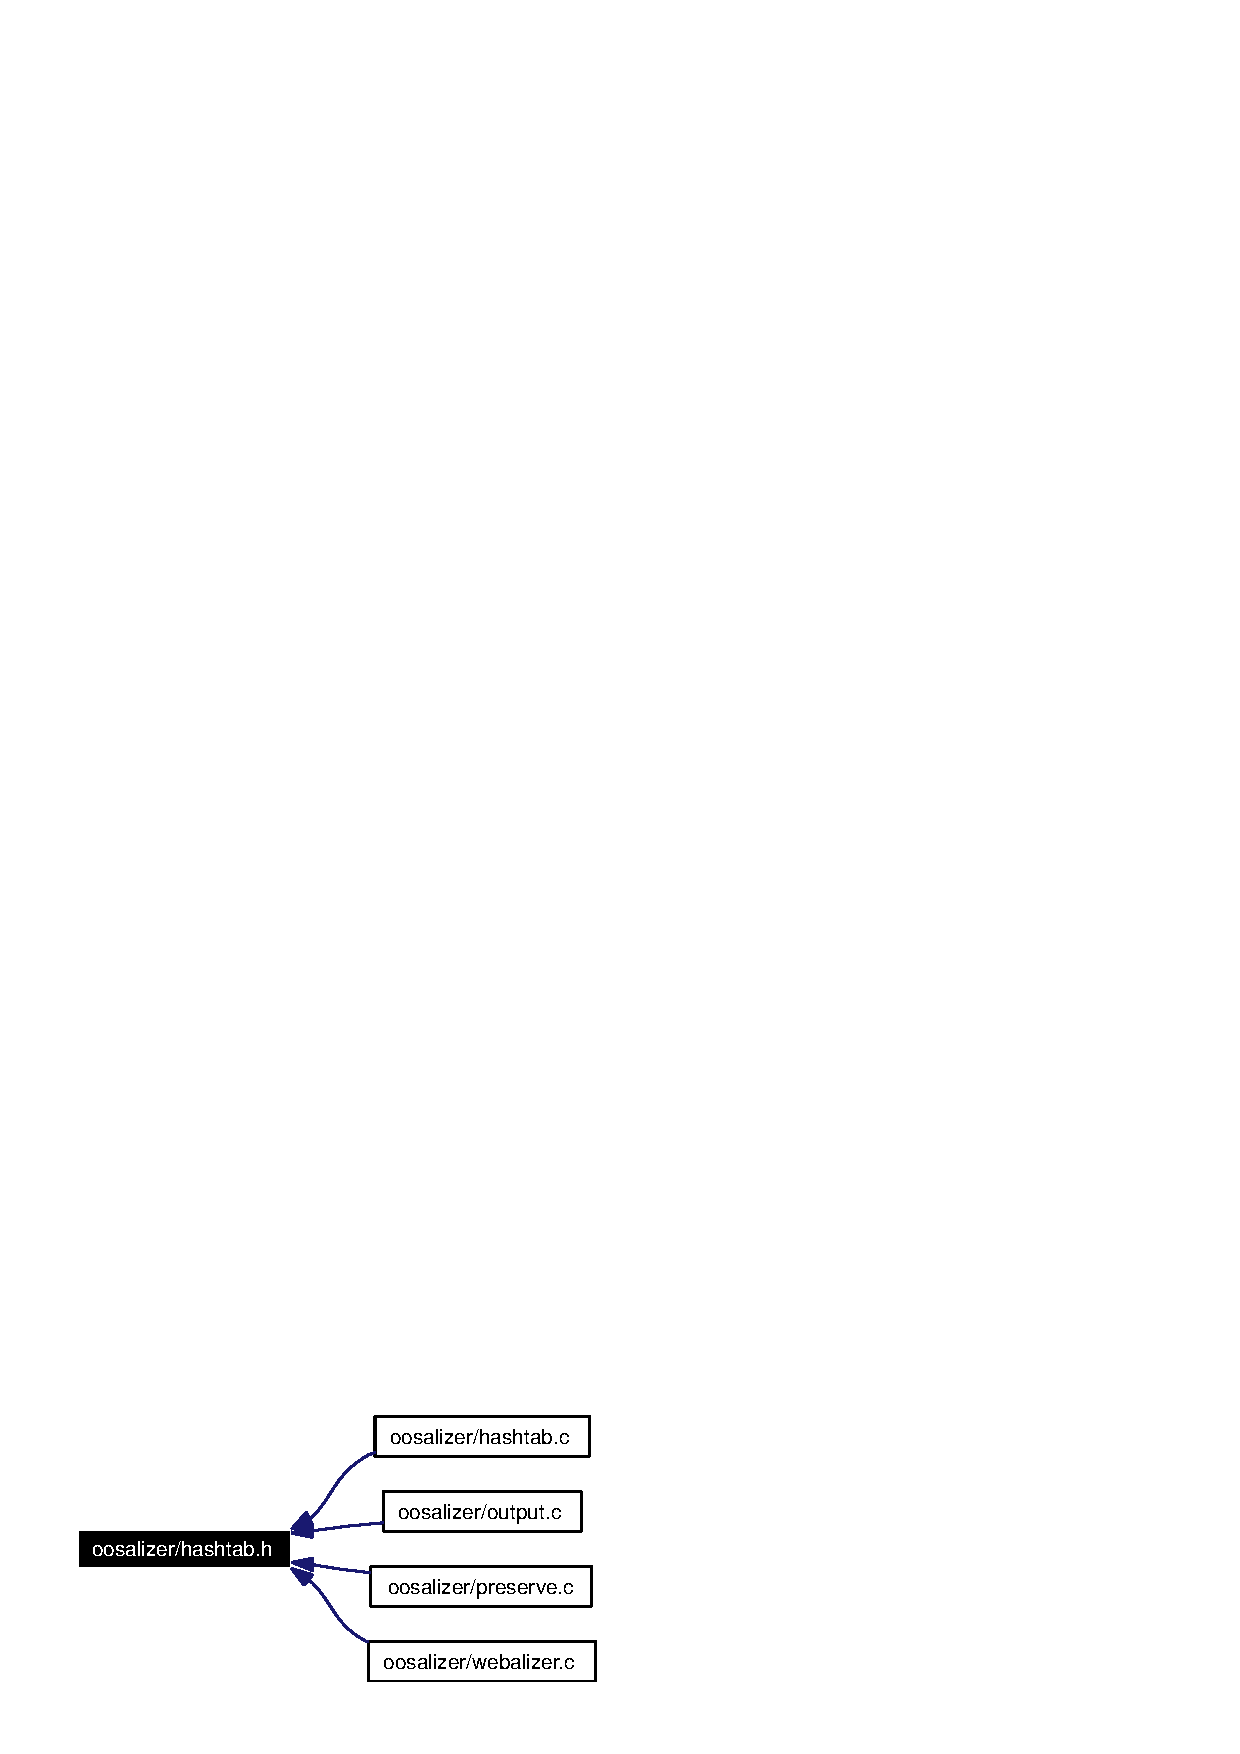
\includegraphics[width=143pt]{hashtab_8h__dep__incl}
\end{center}
\end{figure}
\subsection*{Datenstrukturen}
\begin{CompactItemize}
\item 
struct {\bf hnode}
\item 
struct {\bf unode}
\item 
struct {\bf rnode}
\item 
struct {\bf anode}
\item 
struct {\bf snode}
\item 
struct {\bf inode}
\end{CompactItemize}
\subsection*{Makrodefinitionen}
\begin{CompactItemize}
\item 
\#define {\bf OBJ\_\-REG}~0
\item 
\#define {\bf OBJ\_\-HIDE}~1
\item 
\#define {\bf OBJ\_\-GRP}~2
\end{CompactItemize}
\subsection*{Typdefinitionen}
\begin{CompactItemize}
\item 
typedef {\bf hnode} $\ast$ {\bf HNODEPTR}
\item 
typedef {\bf unode} $\ast$ {\bf UNODEPTR}
\item 
typedef {\bf rnode} $\ast$ {\bf RNODEPTR}
\item 
typedef {\bf anode} $\ast$ {\bf ANODEPTR}
\item 
typedef {\bf snode} $\ast$ {\bf SNODEPTR}
\item 
typedef {\bf inode} $\ast$ {\bf INODEPTR}
\end{CompactItemize}
\subsection*{Funktionen}
\begin{CompactItemize}
\item 
int {\bf put\_\-hnode} (char $\ast$, int, u\_\-long, u\_\-long, double, u\_\-long $\ast$, u\_\-long, u\_\-long, char $\ast$, {\bf HNODEPTR} $\ast$)
\item 
int {\bf put\_\-unode} (char $\ast$, int, u\_\-long, double, u\_\-long $\ast$, u\_\-long, u\_\-long, {\bf UNODEPTR} $\ast$)
\item 
int {\bf put\_\-inode} (char $\ast$, int, u\_\-long, u\_\-long, double, u\_\-long $\ast$, u\_\-long, u\_\-long, {\bf INODEPTR} $\ast$)
\item 
int {\bf put\_\-rnode} (char $\ast$, int, u\_\-long, u\_\-long $\ast$, {\bf RNODEPTR} $\ast$)
\item 
int {\bf put\_\-anode} (char $\ast$, int, u\_\-long, u\_\-long $\ast$, {\bf ANODEPTR} $\ast$)
\item 
int {\bf put\_\-snode} (char $\ast$, u\_\-long, {\bf SNODEPTR} $\ast$)
\item 
void {\bf del\_\-htabs} ()
\item 
void {\bf del\_\-hlist} ({\bf HNODEPTR} $\ast$)
\item 
void {\bf del\_\-ulist} ({\bf UNODEPTR} $\ast$)
\item 
void {\bf del\_\-rlist} ({\bf RNODEPTR} $\ast$)
\item 
void {\bf del\_\-alist} ({\bf ANODEPTR} $\ast$)
\item 
void {\bf del\_\-slist} ({\bf SNODEPTR} $\ast$)
\item 
void {\bf del\_\-ilist} ({\bf INODEPTR} $\ast$)
\item 
void {\bf month\_\-update\_\-exit} (u\_\-long)
\item 
u\_\-long {\bf tot\_\-visit} ({\bf HNODEPTR} $\ast$)
\item 
char $\ast$ {\bf find\_\-url} (char $\ast$)
\end{CompactItemize}
\subsection*{Variablen}
\begin{CompactItemize}
\item 
{\bf HNODEPTR} {\bf sm\_\-htab} [MAXHASH]
\item 
{\bf HNODEPTR} {\bf sd\_\-htab} [MAXHASH]
\item 
{\bf UNODEPTR} {\bf um\_\-htab} [MAXHASH]
\item 
{\bf RNODEPTR} {\bf rm\_\-htab} [MAXHASH]
\item 
{\bf ANODEPTR} {\bf am\_\-htab} [MAXHASH]
\item 
{\bf SNODEPTR} {\bf sr\_\-htab} [MAXHASH]
\item 
{\bf INODEPTR} {\bf im\_\-htab} [MAXHASH]
\end{CompactItemize}


\subsection{Makro-Dokumentation}
\index{hashtab.h@{hashtab.h}!OBJ_GRP@{OBJ\_\-GRP}}
\index{OBJ_GRP@{OBJ\_\-GRP}!hashtab.h@{hashtab.h}}
\subsubsection{\setlength{\rightskip}{0pt plus 5cm}\#define OBJ\_\-GRP~2}\label{hashtab_8h_b2fd3e100a904891f4c27eb46e87140f}




Definiert in Zeile 17 der Datei hashtab.h.

Wird benutzt von all\_\-agents\_\-page(), all\_\-refs\_\-page(), all\_\-sites\_\-page(), all\_\-urls\_\-page(), all\_\-users\_\-page(), dump\_\-all\_\-agents(), dump\_\-all\_\-refs(), dump\_\-all\_\-sites(), dump\_\-all\_\-urls(), dump\_\-all\_\-users(), month\_\-update\_\-exit(), put\_\-anode(), put\_\-hnode(), put\_\-inode(), put\_\-rnode(), put\_\-unode(), top\_\-agents\_\-table(), top\_\-ctry\_\-table(), top\_\-refs\_\-table(), top\_\-sites\_\-table(), top\_\-urls\_\-table(), top\_\-users\_\-table(), tot\_\-visit(), update\_\-entry() und update\_\-exit().\index{hashtab.h@{hashtab.h}!OBJ_HIDE@{OBJ\_\-HIDE}}
\index{OBJ_HIDE@{OBJ\_\-HIDE}!hashtab.h@{hashtab.h}}
\subsubsection{\setlength{\rightskip}{0pt plus 5cm}\#define OBJ\_\-HIDE~1}\label{hashtab_8h_dc29d672dac67a96fe49e055dce78bff}




Definiert in Zeile 16 der Datei hashtab.h.

Wird benutzt von put\_\-anode(), put\_\-hnode(), put\_\-inode(), put\_\-rnode(), put\_\-unode(), top\_\-agents\_\-table(), top\_\-entry\_\-table(), top\_\-refs\_\-table(), top\_\-sites\_\-table(), top\_\-urls\_\-table() und top\_\-users\_\-table().\index{hashtab.h@{hashtab.h}!OBJ_REG@{OBJ\_\-REG}}
\index{OBJ_REG@{OBJ\_\-REG}!hashtab.h@{hashtab.h}}
\subsubsection{\setlength{\rightskip}{0pt plus 5cm}\#define OBJ\_\-REG~0}\label{hashtab_8h_468764de892a2303272613f54f955b0b}




Definiert in Zeile 15 der Datei hashtab.h.

Wird benutzt von all\_\-agents\_\-page(), all\_\-refs\_\-page(), all\_\-sites\_\-page(), all\_\-urls\_\-page(), all\_\-users\_\-page(), new\_\-anode(), new\_\-rnode(), new\_\-unode(), top\_\-agents\_\-table(), top\_\-entry\_\-table(), top\_\-refs\_\-table(), top\_\-sites\_\-table(), top\_\-urls\_\-table() und top\_\-users\_\-table().

\subsection{Dokumentation der benutzerdefinierten Typen}
\index{hashtab.h@{hashtab.h}!ANODEPTR@{ANODEPTR}}
\index{ANODEPTR@{ANODEPTR}!hashtab.h@{hashtab.h}}
\subsubsection{\setlength{\rightskip}{0pt plus 5cm}typedef struct {\bf anode}$\ast$ {\bf ANODEPTR}}\label{hashtab_8h_54e9f1564bf40998b62838a2b06f7798}




Definiert in Zeile 7 der Datei hashtab.h.\index{hashtab.h@{hashtab.h}!HNODEPTR@{HNODEPTR}}
\index{HNODEPTR@{HNODEPTR}!hashtab.h@{hashtab.h}}
\subsubsection{\setlength{\rightskip}{0pt plus 5cm}typedef struct {\bf hnode}$\ast$ {\bf HNODEPTR}}\label{hashtab_8h_6e6c936395602fb2683ed0599131927b}




Definiert in Zeile 4 der Datei hashtab.h.\index{hashtab.h@{hashtab.h}!INODEPTR@{INODEPTR}}
\index{INODEPTR@{INODEPTR}!hashtab.h@{hashtab.h}}
\subsubsection{\setlength{\rightskip}{0pt plus 5cm}typedef struct {\bf inode}$\ast$ {\bf INODEPTR}}\label{hashtab_8h_e88293572818a449e95993c4ccdba0a8}




Definiert in Zeile 9 der Datei hashtab.h.\index{hashtab.h@{hashtab.h}!RNODEPTR@{RNODEPTR}}
\index{RNODEPTR@{RNODEPTR}!hashtab.h@{hashtab.h}}
\subsubsection{\setlength{\rightskip}{0pt plus 5cm}typedef struct {\bf rnode}$\ast$ {\bf RNODEPTR}}\label{hashtab_8h_f93974994603709dc7ef7a9c6798fa23}




Definiert in Zeile 6 der Datei hashtab.h.\index{hashtab.h@{hashtab.h}!SNODEPTR@{SNODEPTR}}
\index{SNODEPTR@{SNODEPTR}!hashtab.h@{hashtab.h}}
\subsubsection{\setlength{\rightskip}{0pt plus 5cm}typedef struct {\bf snode}$\ast$ {\bf SNODEPTR}}\label{hashtab_8h_ba5bd50dc4074b21b1f1cfac70bb1fd5}




Definiert in Zeile 8 der Datei hashtab.h.\index{hashtab.h@{hashtab.h}!UNODEPTR@{UNODEPTR}}
\index{UNODEPTR@{UNODEPTR}!hashtab.h@{hashtab.h}}
\subsubsection{\setlength{\rightskip}{0pt plus 5cm}typedef struct {\bf unode}$\ast$ {\bf UNODEPTR}}\label{hashtab_8h_0d24805080edbea320fb2c2ec31b229a}




Definiert in Zeile 5 der Datei hashtab.h.

\subsection{Dokumentation der Funktionen}
\index{hashtab.h@{hashtab.h}!del_alist@{del\_\-alist}}
\index{del_alist@{del\_\-alist}!hashtab.h@{hashtab.h}}
\subsubsection{\setlength{\rightskip}{0pt plus 5cm}void del\_\-alist ({\bf ANODEPTR} $\ast$)}\label{hashtab_8h_f22586d044db71a37c6df4e122019504}




Definiert in Zeile 645 der Datei hashtab.c.

Benutzt MAXHASH, anode::next und anode::string.

Wird benutzt von del\_\-htabs().\index{hashtab.h@{hashtab.h}!del_hlist@{del\_\-hlist}}
\index{del_hlist@{del\_\-hlist}!hashtab.h@{hashtab.h}}
\subsubsection{\setlength{\rightskip}{0pt plus 5cm}void del\_\-hlist ({\bf HNODEPTR} $\ast$)}\label{hashtab_8h_faa716f0287d99c15c2f1d1b26d74ce0}




Definiert in Zeile 283 der Datei hashtab.c.

Benutzt MAXHASH, hnode::next und hnode::string.

Wird benutzt von del\_\-htabs().\index{hashtab.h@{hashtab.h}!del_htabs@{del\_\-htabs}}
\index{del_htabs@{del\_\-htabs}!hashtab.h@{hashtab.h}}
\subsubsection{\setlength{\rightskip}{0pt plus 5cm}void del\_\-htabs ()}\label{hashtab_8h_f9fcdad76e91434fe5f0728f3a79ae74}




Definiert in Zeile 102 der Datei hashtab.c.

Benutzt am\_\-htab, del\_\-alist(), del\_\-hlist(), del\_\-ilist(), del\_\-rlist(), del\_\-slist(), del\_\-ulist(), im\_\-htab, rm\_\-htab, sd\_\-htab, sm\_\-htab, sr\_\-htab und um\_\-htab.

Wird benutzt von clear\_\-month().\index{hashtab.h@{hashtab.h}!del_ilist@{del\_\-ilist}}
\index{del_ilist@{del\_\-ilist}!hashtab.h@{hashtab.h}}
\subsubsection{\setlength{\rightskip}{0pt plus 5cm}void del\_\-ilist ({\bf INODEPTR} $\ast$)}\label{hashtab_8h_bbc125dd817affa56cc6bcc60c485079}




Definiert in Zeile 918 der Datei hashtab.c.

Benutzt MAXHASH, inode::next und inode::string.

Wird benutzt von del\_\-htabs().\index{hashtab.h@{hashtab.h}!del_rlist@{del\_\-rlist}}
\index{del_rlist@{del\_\-rlist}!hashtab.h@{hashtab.h}}
\subsubsection{\setlength{\rightskip}{0pt plus 5cm}void del\_\-rlist ({\bf RNODEPTR} $\ast$)}\label{hashtab_8h_66b8b1a1eb435b152cb668f00f545a77}




Definiert in Zeile 529 der Datei hashtab.c.

Benutzt MAXHASH, rnode::next und rnode::string.

Wird benutzt von del\_\-htabs().\index{hashtab.h@{hashtab.h}!del_slist@{del\_\-slist}}
\index{del_slist@{del\_\-slist}!hashtab.h@{hashtab.h}}
\subsubsection{\setlength{\rightskip}{0pt plus 5cm}void del\_\-slist ({\bf SNODEPTR} $\ast$)}\label{hashtab_8h_75fb07de23e0c974422e5b44a587dfca}




Definiert in Zeile 750 der Datei hashtab.c.

Benutzt MAXHASH, snode::next und snode::string.

Wird benutzt von del\_\-htabs().\index{hashtab.h@{hashtab.h}!del_ulist@{del\_\-ulist}}
\index{del_ulist@{del\_\-ulist}!hashtab.h@{hashtab.h}}
\subsubsection{\setlength{\rightskip}{0pt plus 5cm}void del\_\-ulist ({\bf UNODEPTR} $\ast$)}\label{hashtab_8h_175d4b20d25d3a0199d63f3bd6a7d0e1}




Definiert in Zeile 410 der Datei hashtab.c.

Benutzt MAXHASH, unode::next und unode::string.

Wird benutzt von del\_\-htabs().\index{hashtab.h@{hashtab.h}!find_url@{find\_\-url}}
\index{find_url@{find\_\-url}!hashtab.h@{hashtab.h}}
\subsubsection{\setlength{\rightskip}{0pt plus 5cm}char$\ast$ find\_\-url (char $\ast$)}\label{hashtab_8h_d3836d00c08459b2f9811d213c4e4550}




Definiert in Zeile 1062 der Datei hashtab.c.

Benutzt blank\_\-str, hash(), unode::next, unode::string und um\_\-htab.

Wird benutzt von put\_\-hnode().\index{hashtab.h@{hashtab.h}!month_update_exit@{month\_\-update\_\-exit}}
\index{month_update_exit@{month\_\-update\_\-exit}!hashtab.h@{hashtab.h}}
\subsubsection{\setlength{\rightskip}{0pt plus 5cm}void month\_\-update\_\-exit (u\_\-long)}\label{hashtab_8h_a516a060c822c1718d2254a425a0c033}




Definiert in Zeile 1136 der Datei hashtab.c.

Benutzt hnode::flag, hnode::lasturl, OBJ\_\-GRP, sm\_\-htab, hnode::tstamp, update\_\-exit() und visit\_\-timeout.\index{hashtab.h@{hashtab.h}!put_anode@{put\_\-anode}}
\index{put_anode@{put\_\-anode}!hashtab.h@{hashtab.h}}
\subsubsection{\setlength{\rightskip}{0pt plus 5cm}int put\_\-anode (char $\ast$, int, u\_\-long, u\_\-long $\ast$, {\bf ANODEPTR} $\ast$)}\label{hashtab_8h_4d9f66275e1a624931142f32f046dd13}




Definiert in Zeile 590 der Datei hashtab.c.

Benutzt anode::count, anode::flag, hash(), hidden\_\-agents, isinlist(), new\_\-anode(), anode::next, OBJ\_\-GRP, OBJ\_\-HIDE und anode::string.\index{hashtab.h@{hashtab.h}!put_hnode@{put\_\-hnode}}
\index{put_hnode@{put\_\-hnode}!hashtab.h@{hashtab.h}}
\subsubsection{\setlength{\rightskip}{0pt plus 5cm}int put\_\-hnode (char $\ast$, int, u\_\-long, u\_\-long, double, u\_\-long $\ast$, u\_\-long, u\_\-long, char $\ast$, {\bf HNODEPTR} $\ast$)}\label{hashtab_8h_fe9c0e49a4926c7cba71b7f8db5db8cd}




Definiert in Zeile 155 der Datei hashtab.c.

Benutzt hnode::count, hnode::files, find\_\-url(), hnode::flag, hash(), hidden\_\-sites, hide\_\-sites, isinlist(), ispage(), hnode::lasturl, log\_\-rec, new\_\-hnode(), hnode::next, OBJ\_\-GRP, OBJ\_\-HIDE, sm\_\-htab, hnode::string, hnode::tstamp, update\_\-entry(), update\_\-exit(), log\_\-struct::url, hnode::visit, visit\_\-timeout und hnode::xfer.\index{hashtab.h@{hashtab.h}!put_inode@{put\_\-inode}}
\index{put_inode@{put\_\-inode}!hashtab.h@{hashtab.h}}
\subsubsection{\setlength{\rightskip}{0pt plus 5cm}int put\_\-inode (char $\ast$, int, u\_\-long, u\_\-long, double, u\_\-long $\ast$, u\_\-long, u\_\-long, {\bf INODEPTR} $\ast$)}\label{hashtab_8h_62c7ecc5b3ae3851f5400e30734b8e9e}




Definiert in Zeile 811 der Datei hashtab.c.

Benutzt inode::count, inode::files, inode::flag, hash(), hidden\_\-users, isinlist(), ispage(), log\_\-rec, new\_\-inode(), inode::next, OBJ\_\-GRP, OBJ\_\-HIDE, inode::string, inode::tstamp, log\_\-struct::url, inode::visit, visit\_\-timeout und inode::xfer.\index{hashtab.h@{hashtab.h}!put_rnode@{put\_\-rnode}}
\index{put_rnode@{put\_\-rnode}!hashtab.h@{hashtab.h}}
\subsubsection{\setlength{\rightskip}{0pt plus 5cm}int put\_\-rnode (char $\ast$, int, u\_\-long, u\_\-long $\ast$, {\bf RNODEPTR} $\ast$)}\label{hashtab_8h_cba57da4379852348b455ce6e86ef96b}




Definiert in Zeile 471 der Datei hashtab.c.

Benutzt rnode::count, rnode::flag, hash(), hidden\_\-refs, isinlist(), new\_\-rnode(), rnode::next, OBJ\_\-GRP, OBJ\_\-HIDE und rnode::string.\index{hashtab.h@{hashtab.h}!put_snode@{put\_\-snode}}
\index{put_snode@{put\_\-snode}!hashtab.h@{hashtab.h}}
\subsubsection{\setlength{\rightskip}{0pt plus 5cm}int put\_\-snode (char $\ast$, u\_\-long, {\bf SNODEPTR} $\ast$)}\label{hashtab_8h_e9754e3f6f6b9926edb3bf1706f8202a}




Definiert in Zeile 705 der Datei hashtab.c.

Benutzt snode::count, hash(), new\_\-snode(), snode::next und snode::string.

Wird benutzt von srch\_\-string().\index{hashtab.h@{hashtab.h}!put_unode@{put\_\-unode}}
\index{put_unode@{put\_\-unode}!hashtab.h@{hashtab.h}}
\subsubsection{\setlength{\rightskip}{0pt plus 5cm}int put\_\-unode (char $\ast$, int, u\_\-long, double, u\_\-long $\ast$, u\_\-long, u\_\-long, {\bf UNODEPTR} $\ast$)}\label{hashtab_8h_96366abcaec7b7275725bb40618976ab}




Definiert in Zeile 344 der Datei hashtab.c.

Benutzt unode::count, unode::entry, unode::exit, unode::flag, hash(), hidden\_\-urls, isinlist(), new\_\-unode(), unode::next, OBJ\_\-GRP, OBJ\_\-HIDE, unode::string und unode::xfer.\index{hashtab.h@{hashtab.h}!tot_visit@{tot\_\-visit}}
\index{tot_visit@{tot\_\-visit}!hashtab.h@{hashtab.h}}
\subsubsection{\setlength{\rightskip}{0pt plus 5cm}u\_\-long tot\_\-visit ({\bf HNODEPTR} $\ast$)}\label{hashtab_8h_4bdcfce12ca5e5236241cfdd1ec5288a}




Definiert in Zeile 1160 der Datei hashtab.c.

Benutzt hnode::flag, MAXHASH, hnode::next, OBJ\_\-GRP und hnode::visit.

\subsection{Variablen-Dokumentation}
\index{hashtab.h@{hashtab.h}!am_htab@{am\_\-htab}}
\index{am_htab@{am\_\-htab}!hashtab.h@{hashtab.h}}
\subsubsection{\setlength{\rightskip}{0pt plus 5cm}{\bf ANODEPTR} {\bf am\_\-htab}[MAXHASH]}\label{hashtab_8h_4886dbd661ad553906dc83e1a8031316}




Definiert in Zeile 90 der Datei hashtab.c.

Wird benutzt von del\_\-htabs() und load\_\-agent\_\-array().\index{hashtab.h@{hashtab.h}!im_htab@{im\_\-htab}}
\index{im_htab@{im\_\-htab}!hashtab.h@{hashtab.h}}
\subsubsection{\setlength{\rightskip}{0pt plus 5cm}{\bf INODEPTR} {\bf im\_\-htab}[MAXHASH]}\label{hashtab_8h_1a7bfe1ecf3b78722bcee9d08e8178a1}




Definiert in Zeile 92 der Datei hashtab.c.

Wird benutzt von del\_\-htabs() und load\_\-ident\_\-array().\index{hashtab.h@{hashtab.h}!rm_htab@{rm\_\-htab}}
\index{rm_htab@{rm\_\-htab}!hashtab.h@{hashtab.h}}
\subsubsection{\setlength{\rightskip}{0pt plus 5cm}{\bf RNODEPTR} {\bf rm\_\-htab}[MAXHASH]}\label{hashtab_8h_4b36877a2219872c641eb9a58ae45ce8}




Definiert in Zeile 89 der Datei hashtab.c.

Wird benutzt von del\_\-htabs() und load\_\-ref\_\-array().\index{hashtab.h@{hashtab.h}!sd_htab@{sd\_\-htab}}
\index{sd_htab@{sd\_\-htab}!hashtab.h@{hashtab.h}}
\subsubsection{\setlength{\rightskip}{0pt plus 5cm}{\bf HNODEPTR} {\bf sd\_\-htab}[MAXHASH]}\label{hashtab_8h_e5ddad8435a9d403e79f4bd320fea151}




Definiert in Zeile 87 der Datei hashtab.c.

Wird benutzt von del\_\-htabs().\index{hashtab.h@{hashtab.h}!sm_htab@{sm\_\-htab}}
\index{sm_htab@{sm\_\-htab}!hashtab.h@{hashtab.h}}
\subsubsection{\setlength{\rightskip}{0pt plus 5cm}{\bf HNODEPTR} {\bf sm\_\-htab}[MAXHASH]}\label{hashtab_8h_408742678920fdb90b2926c215e8e19c}




Definiert in Zeile 86 der Datei hashtab.c.

Wird benutzt von del\_\-htabs(), load\_\-site\_\-array(), month\_\-update\_\-exit(), put\_\-hnode() und top\_\-ctry\_\-table().\index{hashtab.h@{hashtab.h}!sr_htab@{sr\_\-htab}}
\index{sr_htab@{sr\_\-htab}!hashtab.h@{hashtab.h}}
\subsubsection{\setlength{\rightskip}{0pt plus 5cm}{\bf SNODEPTR} {\bf sr\_\-htab}[MAXHASH]}\label{hashtab_8h_e9a8ef54a4b421e3d16dc313f162ccff}




Definiert in Zeile 91 der Datei hashtab.c.

Wird benutzt von del\_\-htabs(), load\_\-srch\_\-array() und srch\_\-string().\index{hashtab.h@{hashtab.h}!um_htab@{um\_\-htab}}
\index{um_htab@{um\_\-htab}!hashtab.h@{hashtab.h}}
\subsubsection{\setlength{\rightskip}{0pt plus 5cm}{\bf UNODEPTR} {\bf um\_\-htab}[MAXHASH]}\label{hashtab_8h_2f99d64abd1711a4b10ee71d070811a7}




Definiert in Zeile 88 der Datei hashtab.c.

Wird benutzt von del\_\-htabs(), find\_\-url(), load\_\-url\_\-array(), update\_\-entry() und update\_\-exit().